\chapter{目标代码生成}

前面的章节中,我们已经建构了抽象语法树 (AST),并进行了类型检查。在此基础上,我们需要通过抽象语法树生成目标代码。

尽管我们的确可以从抽象语法树直接生成目标平台的代码,然而现实情况并非如此。假设我们有
$m$ 门语言,$n$ 个目标平台,那么如果采用直接生成代码,则需要写 $m\times n$
个转换程序,这对于现代编译器来说是无法承受的。但是如果我们选取一门中间语言作为转换的中转,那么我只要实现
$m$ 个从语言到中间语言的转换程序,以及 $n$ 个从中间语言到目标平台的转换程序,就可以满足需求。这样的中间语言被称为
IR (intermediate representation)。此外,对于后续的优化,也可以在 IR 上处理,这可以大大减少编译器优化工作。

本章中,我们以 LLVM Language (version 15) 为例,来展示如何从中间语言转换成目标代码。如需查看
LLVM 的完整文档,请访问 \url{https://llvm.org/docs/LangRef.html}。

\begin{remark}
本章涉及程序链接的一部分内容。在阅读本章前,强烈建议先行了解关于链接器 (linker) 的知识
(维基百科链接:\url{https://en.wikipedia.org/wiki/Linker_(computing)})。
\end{remark}

\section{LLVM 15 概览}

LLVM 是一套编译器基础设施项目,包含一系列模块化的编译器组件和工具链,用来开发编译器前端和后端。

IR 是区分前后端的标志。语法检查、建构抽象语法树、生成 IR 都属于前端部分。通过 IR
生成目标代码、针对 IR 层面的优化都属于后端部分。

LLVM 提供的工具链可以检查 IR 问题、运行及调试 IR,因此我们推荐使用 LLVM IR
作为我们编译器的 IR。

LLVM 项目中有很多非常实用的工具——如 clang、llc、lli 等等。一般来是,最常用的工具是
clang,因为 clang 可以将代码编译到 LLVM IR,也可以将 LLVM 代码编译到目标平台。比如
\texttt{clang main.c -S -emit-llvm --target=riscv32-unknown-elf -o main.ll}
可以将 \texttt{main.c} 转换成 LLVM IR 并保存在 \texttt{main.ll} 中;而
\texttt{clang -S main.ll --target=riscv32-unknown-elf -o main.s}
可以将 \texttt{main.ll} 转换成汇编。llc 可以将 LLVM IR 转换成汇编,如
\texttt{llc -march=riscv32 main.ll -o main.s} 会将 \texttt{main.ll}
转换成汇编并存到 \texttt{main.s}。

LLVM IR 语言与高级语言不同,不存在多层嵌套的环境,指令以基础块 (basic block)
的形式组织,与汇编语言非常相近,同时又保留了高级语言的类型属性。选择 LLVM 15
的原因是从 LLVM 15 开始,LLVM IR 默认使用不透明指针
(Opaque Pointers),大大减少了转换时的负担。具体请参见章节 \ref{LLVM-semantic}。

LLVM IR 的一大特性是静态单赋值 (Static Single Assignment,
SSA),即变量能且仅能被赋值一次,这一特性可以让编译器的静态分析更方便。

当然,你也可以使用其他 IR 或是直接一步从 AST
转换成目标代码(因为我们的编译器只有一个目标平台)。

\section{LLVM 15 环境}

\subsection{在线 LLVM 环境}\label{online-LLVM-env}

在学习 LLVM 的过程中,一个方便的使用环境非常重要。Godbolt (
\url{https://godbolt.org/}) 提供了几乎所有的编译器,并且可以编译到大量平台。

\begin{figure}[htb]
\centering
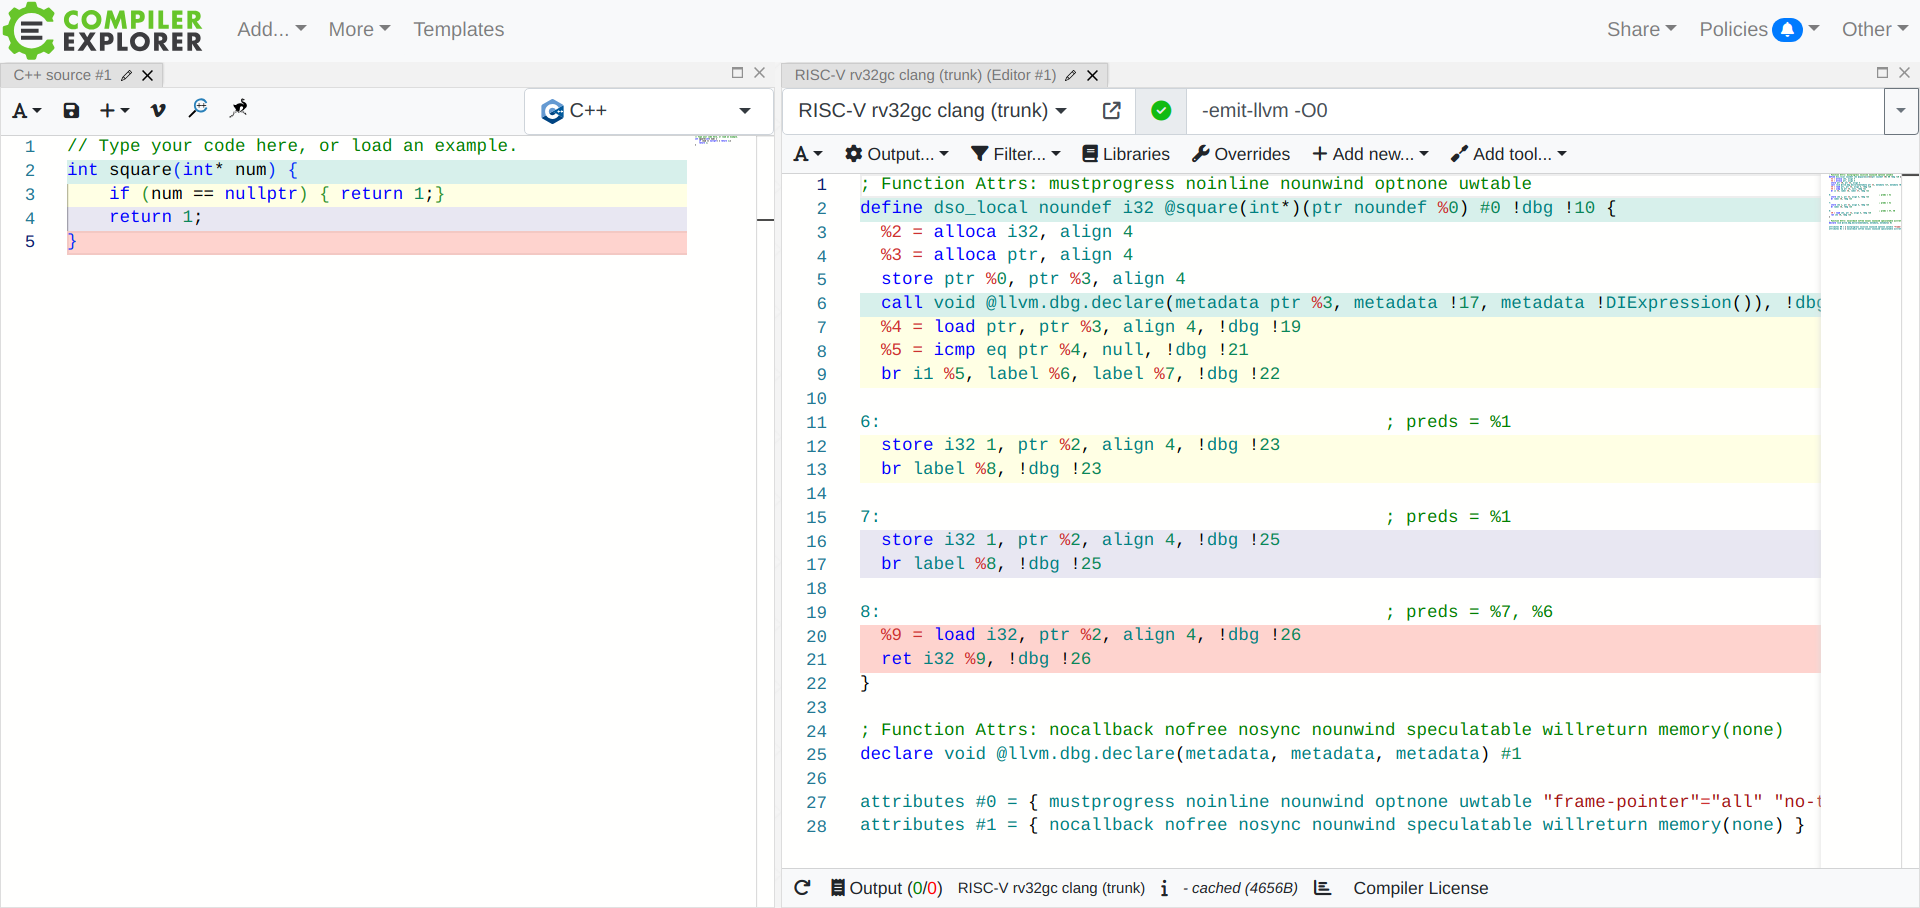
\includegraphics[scale=0.3]{image/godbolt.png}
\caption{Godbolt 使用截图}
\label{godbolt_sreenshot}
\end{figure}

图片 \ref{godbolt_sreenshot} 是一个通过在线 LLVM 环境来了解 LLVM 语言的例子。在
gofbolt 上,页面被分为两栏——左栏是你的输入,右栏是你选择的编译器在你填入的参数下的输入。下面我们将会分别介绍左右栏的使用。

左栏有一个语言选择框(位于左栏的上部)和一个代码输入框。语言选择框可以选择所使用的编程语言。

右栏上部左边部分是编译器选择框,右边部分是编译器参数框。我们此时希望将代码编译到适用于 rv32gc
平台的 LLVM 语言,而且不希望编译器做出优化(否则可能会把一部分代码直接去掉)。由于我们的编译器的目标平台是
rv32gc,且 clang 可以通过 \texttt{-emit-llvm} 来输出 LLVM 语言,因此我们在编译器选择框选择
RISCV rv32gc clang (trunk)(trunk 这里表示最新的 clang),在编译器参数框中输入 \texttt{-emit-llvm -O0}。

关于语言特性的内容,请见章节 \ref{LLVM-semantic}。

\subsection{本地 LLVM 环境}

你可以安装 LLVM 15 及其以上版本。截止 LLVM 17,所有的 LLVM 15 特性均可使用。

对于使用 apt 包管理的用户(debian/Ubuntu/... 用户),请参考 \href{https://apt.llvm.org/}{LLVM apt 安装文档}。

对于使用 pacman 包管理的用户,可以执行 \texttt{sudo pacman -S llvm clang} 安装最新版本的 LLVM。

你可以执行 \texttt{clang --version} 来检查 clang 15 及以上版本是否确实安装到系统中。
正常情况下,该指令会显示你的 clang 版本、目标平台等信息。你需要检查对应的版本是否正确。

\begin{remark}
如果你用的是特定版本的 LLVM(而非最新版本),在使用程序时,需要加上 \texttt{-<version>} 后缀。比如 \texttt{clang-15 ...}。
\end{remark}

\section{LLVM 15 语法}\label{LLVM-semantic}

\begin{remark}
本章节只介绍常用的 LLVM 15 语法。如需了解全部语法或更详细的 LLVM 语法,请访问
\url{https://llvm.org/docs/LangRef.html}。
\end{remark}

\begin{remark}
你可以先大致了解 LLVM 15 语法,然后跳到「从抽象语法树到中间语言」章节
(\ref{AST-to-IR}) 了解如何完成抽象语法树到 IR
的转换。在阅读「从抽象语法树到中间语言」部分的过程中,如果对 LLVM IR
的语法有疑惑,再回到本部分查看详细信息。
\end{remark}

\subsection{LLVM 15 简单例子}

对于下面的代码,
\begin{lstlisting}[language=C]
int c;
int foo(int* a, int b) {
    if (a == 0) return 0;
    return  *a + b + c;
}
\end{lstlisting}

在 \texttt{-emit-llvm -O1 -fno-discard-value-names}
参数下,会生成下面的代码(下面的代码去掉了生成代码的 attribute
部分和一些注释,这些内容我们在编译器大作业中应该用不到)

\begin{lstlisting}[language=llvm]
@c = dso_local local_unnamed_addr global i32 0, align 4, !dbg !0

define dso_local i32 @foo(ptr noundef readonly %a, i32 noundef %b) local_unnamed_addr #0 !dbg !15 {
entry:
  call void @llvm.dbg.value(metadata ptr %a, metadata !20, metadata !DIExpression()), !dbg !22
  call void @llvm.dbg.value(metadata i32 %b, metadata !21, metadata !DIExpression()), !dbg !22
  %cmp = icmp eq ptr %a, null, !dbg !23
  br i1 %cmp, label %return, label %if.end, !dbg !25

if.end:                                           ; preds = %entry
  %0 = load i32, ptr %a, align 4, !dbg !26
  %add = add nsw i32 %0, %b, !dbg !31
  %1 = load i32, ptr @c, align 4, !dbg !32
  %add1 = add nsw i32 %add, %1, !dbg !33
  br label %return, !dbg !34

return:                                           ; preds = %entry, %if.end
  %retval.0 = phi i32 [ %add1, %if.end ], [ 0, %entry ], !dbg !22
  ret i32 %retval.0, !dbg !35
}
\end{lstlisting}

进一步地,我们还可以忽略一些 debug 参数、一些无用的参数(如
\texttt{dso\_local}、\texttt{local\_unnamed\_addr} 和
\texttt{align})以及不必要的 debug 函数,这样可以得到以下的代码

\begin{lstlisting}[language=llvm]
@c = global i32 0

define i32 @foo(ptr %a, i32 %b) {
entry:
  %cmp = icmp eq ptr %a, null
  br i1 %cmp, label %return, label %if.end

if.end:                       ; preds = %entry
  %0 = load i32, ptr %a
  %add = add i32 %0, %b
  %1 = load i32, ptr @c
  %add1 = add i32 %add, %1
  br label %return

return:                       ; preds = %entry, %if.end
  %retval.0 = phi i32 [ %add1, %if.end ], [ 0, %entry ]
  ret i32 %retval.0
}
\end{lstlisting}

我们会在本章每个元素一一解释。如果你设置了 \texttt{-O0},你会看到一些如
\texttt{\%3 = alloca i32} 的指令,我们也会在本章中介绍。

\subsection{LLVM 15 基本语法}

LLVM 15 的基本语法包含
\begin{itemize}
  \item 类型,如 \texttt{i1},\texttt{i32},具体参见章节 \ref{LLVM-types};
  \item 变量,如 \texttt{@a = global i32 0} 以及
    \texttt{\%a = ...},具体参见章节 \ref{LLVM-variables};
  \item 常量,具体参见章节 \ref{LLVM-constants};
  \item 函数定义及声明,如 \texttt{define i32 \@foo(ptr \%0, i32 \%1) \{...\}},具体参见章节
    \ref{LLVM-functions};
  \item 标签 (label),如 \texttt{4:};
  \item 指令,如 \texttt{\%3 = icmp eq ptr \%0, null},具体参见章节
    \ref{LLVM-instructions}。
\end{itemize}

一个基本的 LLVM IR 翻译单元由若干类型声明、若干全局变量和若干函数定义组成。

函数定义由若干标签和若干指令组成。标签是可以被分支指令 (\ref{LLVM-br-instructions})
跳转到的地方。在函数外部的变量为全局变量,在函数内部的变量为局部变量。
所有的变量能且仅能被赋值一次(因此全局变量实际上是指向变量的指针)。

每行的分号 (\texttt{;}) 后的内容为注释。如没有注释,分号是不必要的。

\subsection{类型}\label{LLVM-types}

常用的类型有
\begin{itemize}
  \item 整数类型:用 \texttt{i<N>} 表示,如 \texttt{i32},\texttt{i1},
    注意整型的长度与内存中的对齐没有必然的联系,\texttt{i1} 是 1 bit 长,不代表八个 \texttt{i1}
    占用 1 byte;
  \item 指针类型:用 \texttt{ptr} 表示;
  \item 数组类型:用 \texttt{[<\# elements> x <elementtype>]} 表示,如
    \texttt{[40 x i32]}。数组类型允许嵌套定义,如
    \texttt{[3 x [4 x i32]]},表示 $3\times 4$ 的二维数组。另请参见
    \url{https://llvm.org/docs/LangRef.html#array-type};
  \item 结构类型:对于普通的类,用 \texttt{\%<typename> = type \{ <type list> \}} 表示,如
    \texttt{\%mytype = type \{ \%mytype*, i32 \}};对于不能对齐的类
    (packed struct),用 \texttt{\%<typename> = type <\{ <type list> \}>}
    表示,如 \texttt{<\{ i8, i32 \}>} 表示一个 5 字节的结构体。
\end{itemize}

\subsection{变量}\label{LLVM-variables}

非匿名变量的命名必须符合 \texttt{[\%@][-a-zA-Z\$.\_][-a-zA-Z\$.\_0-9]*},且不能与作用域中的其他变量名或函数名冲突。

匿名变量的命名必须符合 \texttt{[\%@](0|[1-9][0-9]*)},且不能与作用域中的其他变量名或函数名冲突。

变量分为全局变量和局部变量。全局变量以 \texttt @ 开头,如 \texttt{@abc};局部变量以 \texttt \% 开头,如 \texttt{\%abc}。

变量能且只能被赋值一次。

\subsection{常量}\label{LLVM-constants}

常量有
\begin{itemize}
  \item boolean 常量: 仅有 \texttt{true},\texttt{false} 两个字符串,类型为 \texttt{i1}。
  \item int 常量:支持所有标准的整数。
  \item 空指针常量:仅支持字符串 \texttt{null},类型为 \texttt{ptr}。
\end{itemize}

\begin{remark}
如需使用其他常量,请参见\href{https://llvm.org/docs/LangRef.html\#constants}{官方文档}。
\end{remark}

\subsection{函数定义及声明}\label{LLVM-functions}

函数的定义方式如下:

\begin{lstlisting}[language=llvm]
define <ResultType> @<FunctionName>(...) { ... }
\end{lstlisting}

圆括号内为函数参数,参数用逗号分割,每项参数的形式为 \texttt{<type> [name]}。

典型的例子有:
\begin{itemize}
  \item 无入参函数 \texttt{int a()},对应的函数为 \texttt{define i32 \@a() \{...\}};
  \item 单入参函数 \texttt{void a(int x)},对应的函数为 \texttt{define void \@a(i32 \%x) \{...\}};
  \item 双入参函数 \texttt{int a(int x1, int x2)},
    对应的函数为 \texttt{define i32 \@a(i32 \%x1, i32 \%x2) \{...\}}。
\end{itemize}

花括号内为函数的指令以及若干标签 (label)。

函数的声明方式如下:

\begin{lstlisting}[language=llvm]
declare <ResultType> @<FunctionName>(...)
\end{lstlisting}

声明的形式基本上和定义一致,只不过去掉了函数体,前面的 \texttt{define} 被换成了
\texttt{declare}。

\begin{remark}
关于函数调用,请参见 call 指令 (\ref{LLVM-call-instructions})。
\end{remark}

\subsection{指令}\label{LLVM-instructions}

\begin{remark}
以下的介绍中的语法只是 LLVM IR 语法的一部分。关于全部语法,请访问
\url{https://llvm.org/docs/LangRef.html\#instruction-reference}。
同时,每个指令的章节也会附上对应的官方文档链接。
\end{remark}

在 LLVM IR 中,我们一般会用到以下指令:(点击括号中的章节号可以跳转到对应章节)

\begin{itemize}
  \item 二元运算指令 (\ref{LLVM-binary-instructions})
    \begin{itemize}
      \item \texttt{add} 指令
      \item \texttt{sub} 指令
      \item \texttt{mul} 指令
      \item \texttt{sdiv} 指令
      \item \texttt{srem} 指令
      \item \texttt{shl} 指令
      \item \texttt{ashr} 指令
      \item \texttt{and} 指令
      \item \texttt{or} 指令
      \item \texttt{xor} 指令
    \end{itemize}
  \item 控制流相关指令
    \begin{itemize}
      \item \texttt{br} 指令 (\ref{LLVM-br-instructions})
      \item \texttt{ret} 指令 (\ref{LLVM-ret-instructions})
    \end{itemize}
  \item 内存相关指令
    \begin{itemize}
      \item \texttt{alloca} 指令 (\ref{LLVM-alloca-instructions})
      \item \texttt{load} 指令 (\ref{LLVM-load-instructions})
      \item \texttt{store} 指令 (\ref{LLVM-store-instructions})
      \item \texttt{getelementptr} 指令 (\ref{LLVM-gep-instructions})
    \end{itemize}
  \item 其他指令
    \begin{itemize}
      \item \texttt{icmp} 指令 (\ref{LLVM-icmp-instructions})
      \item \texttt{call} 指令 (\ref{LLVM-call-instructions})
      \item \texttt{phi} 指令 (\ref{LLVM-phi-instructions})
    \end{itemize}
\end{itemize}

\subsubsection{二元运算指令}\label{LLVM-binary-instructions}

\begin{remark}
完整文档位于 \url{https://llvm.org/docs/LangRef.html\#binary-operations}。
\end{remark}

语法:
\begin{lstlisting}[language=llvm]
<result> = <operator> <type> <operand1>, <operand2>
\end{lstlisting}

支持的运算符(对应形式中的 \texttt{operator})有:
\begin{itemize}
  \item add:整数加法
  \item sub:整数减法
  \item mul:整数乘法
  \item sdiv:有符号整数除法
  \item srem:有符号整数取模
  \item shl:左移
  \item ashr:算术右移
  \item and:按位与
  \item or:按位或
  \item xor:异或
\end{itemize}

例子:
\begin{lstlisting}[language=llvm]
%_add_result_1 = add i32 %a, %b
\end{lstlisting}

该指令表示将 \texttt{\%a} 与 \texttt{\%b} 之和存入 \texttt{\%\_add\_result\_1}。

\subsubsection{\texttt{br} 指令}\label{LLVM-br-instructions}

\begin{remark}
完整文档位于 \url{https://llvm.org/docs/LangRef.html\#br-instruction}。
\end{remark}

语法:
\begin{lstlisting}[language=llvm]
br i1 <cond>, label <iftrue>, label <iffalse> ; Conditional branch
br label <dest> ; Unconditional branch
\end{lstlisting}

\begin{itemize}
  \item \texttt{cond} 必须是一个 \texttt{i1} 类型的变量;
  \item \texttt{iftrue}、\texttt{iffalse} 以及 \texttt{dest}
    必须是所在函数里的一个标签;
  \item 由于 \texttt{br} 指令的下一个执行的指令一定不是下一条指令,因此一个基础块
    (basic block) 里的指令中 \texttt{br} 之后的指令是没有意义的。
\end{itemize}

例子:
\begin{lstlisting}[language=llvm]
br i1 %a, label %label_1, label %label_2 ; Conditional branch
br label %label_3 ; Unconditional branch
\end{lstlisting}

第 1 行表示如果 \texttt{\%a} 是 \texttt{true},则跳转到
\texttt{label\_1},否则跳转到 \texttt{label\_2}。第 2 行表示直接跳转到
\texttt{label\_3}。

\subsubsection{\texttt{ret} 指令}\label{LLVM-ret-instructions}

\begin{remark}
完整文档位于 \url{https://llvm.org/docs/LangRef.html\#ret-instruction}。
\end{remark}

语法:
\begin{lstlisting}[language=llvm]
ret <type> <value> ; Return a value from a non-void function
ret void ; Return from void function
\end{lstlisting}

\begin{itemize}
  \item \texttt{value} 的类型必须与 \texttt{type} 和函数的返回类型相同;
  \item 与 \texttt{br} 指令类似,一个基础块里的 \texttt{ret}
    指令之后的所有指令都不可达,因此都没有意义。
\end{itemize}

例子:
\begin{lstlisting}[language=llvm]
ret ptr %a
ret i32 1
\end{lstlisting}

第 1 行表示返回 \texttt{\%a}。第 2 行表示返回一个常数 1。

\subsubsection{\texttt{alloca} 指令}\label{LLVM-alloca-instructions}

\begin{remark}
完整文档位于 \url{https://llvm.org/docs/LangRef.html\#alloca-instruction}。
\end{remark}

语法:
\begin{lstlisting}[language=llvm]
<result> = alloca <type>
\end{lstlisting}

\begin{itemize}
  \item \texttt{alloca} 指令可以在当前函数的栈上为 \texttt{type} 类型分配一块的内存空间;
  \item \texttt{result} 是指向该空间的指针,类型是指针类型 (\texttt{ptr})。
\end{itemize}

例子:
\begin{lstlisting}[language=llvm]
%ptr_1 = alloca i32
\end{lstlisting}
表示在当前函数的栈上分配一块 \texttt{sizeof(i32)} 字节的空间,\texttt{\%ptr\_1} 指向该空间。

\subsubsection{\texttt{load} 指令}\label{LLVM-load-instructions}

\begin{remark}
完整文档位于 \url{https://llvm.org/docs/LangRef.html\#load-instruction}。
\end{remark}

语法:
\begin{lstlisting}[language=llvm]
<result> = load <ty>, ptr <pointer>
\end{lstlisting}

\begin{itemize}
  \item \texttt{result} 的类型是 \texttt{ty};
  \item \texttt{result} 被赋值为 \texttt{pointer} 所指向的值。
\end{itemize}

例子:
\begin{lstlisting}[language=llvm]
%ptr = alloca i32
store i32 3, ptr %ptr
%val = load i32, ptr %ptr
\end{lstlisting}

第 3 行表示将 \texttt{\%ptr} 所指向的值赋值给 \texttt{\%val},此处 \texttt{\%val}
的值为 3。

\subsubsection{\texttt{store} 指令}\label{LLVM-store-instructions}

\begin{remark}
完整文档位于 \url{https://llvm.org/docs/LangRef.html\#store-instruction}。
\end{remark}

语法:
\begin{lstlisting}[language=llvm]
store <ty> <value>, ptr <pointer>
\end{lstlisting}

\begin{itemize}
  \item \texttt{pointer} 所指向的值会被赋值为 \texttt{value}。
\end{itemize}

例子:
\begin{lstlisting}[language=llvm]
%ptr = alloca i32
store i32 3, ptr %ptr
%val = load i32, ptr %ptr
\end{lstlisting}

第 2 行表示将 \texttt{\%ptr} 所指向的值赋值为 3。因此第 3 行中,\texttt{\%val}
的值为 3。

\subsubsection{\texttt{getelementptr} 指令}\label{LLVM-gep-instructions}

\begin{remark}
完整文档位于 \url{https://llvm.org/docs/LangRef.html\#getelementptr-instruction}。
\end{remark}

在编译器大作业中,以下的语法可以胜任全部要求:
\begin{lstlisting}[language=llvm]
<result> = getelementptr <ty>, ptr <ptrval>{, <ty> <idx>}*
\end{lstlisting}

\texttt{getelementptr} 指令较为复杂,我们先看一个例子。

对于以下的 C 代码:
\begin{lstlisting}[language=C]
struct RT {
  char A;
  int B[10][20];
  char C;
};
struct ST {
  int X;
  double Y;
  struct RT Z;
};

int *foo(struct ST *s) {
  return &s[1].Z.B[5][13];
}
\end{lstlisting}
对应的 LLVM IR 为
\begin{lstlisting}[language=llvm]
%struct.RT = type { i8, [10 x [20 x i32]], i8 }
%struct.ST = type { i32, double, %struct.RT }

define ptr @foo(ptr %s) {
entry:
  %arrayidx = getelementptr %struct.ST, ptr %s, i64 1, i32 2, i32 1, i64 5, i64 13
  ret ptr %arrayidx
}
\end{lstlisting}

可以发现 \texttt{getelementptr} 指令会对类型逐层解析。将 ST 的指针先取下标为 1 的元素,然后访问成员
\texttt{Z}。由于成员是 \texttt{ST} 的第 2 个元素 (0-based),因此取下标 2。接下来是取成员
\texttt{B},同理由于其为第 1 个元素,取下标 1。\texttt{B} 的类型为一个二维数组,因此取下标 5 后再取下标 13
即可获得所需的指针。

上面的代码与下面的代码(逐步解引用)等价:
\begin{lstlisting}[language=llvm]
%struct.RT = type { i8, [10 x [20 x i32]], i8 }
%struct.ST = type { i32, double, %struct.RT }

define ptr @foo(ptr %s) {
  %t1 = getelementptr %struct.ST, ptr %s, i32 1
  %t2 = getelementptr %struct.ST, ptr %t1, i32 0, i32 2
  %t3 = getelementptr %struct.RT, ptr %t2, i32 0, i32 1
  %t4 = getelementptr [10 x [20 x i32]], ptr %t3, i32 0, i32 5
  %t5 = getelementptr [20 x i32], ptr %t4, i32 0, i32 13
  ret ptr %t5
}
\end{lstlisting}

\begin{itemize}
  \item \texttt{ty} 为 \texttt{ptrval} 所指向内容的类型,因此
    \texttt{\%t1 = getelementptr \%struct.ST, ptr \%p, i32 5}
    表示通过 \texttt{\%struct.ST} 指针获得指向第 5 个 \texttt{ST}
    的指针(如果需要访问的是指针指向的第 5 个元素,则应当使用
    \texttt{\%t1 = getelementptr \%struct.ST, ptr \%p, i32 0, i32 5};
  \item \texttt{result} 为指向对应成员的指针(一定要注意这一点);
  \item 为了方便编写代码,推荐逐步解引用。
\end{itemize}

\subsubsection{\texttt{icmp} 指令}\label{LLVM-icmp-instructions}

\begin{remark}
完整文档位于 \url{https://llvm.org/docs/LangRef.html\#icmp-instruction}。
\end{remark}

语法:
\begin{lstlisting}[language=llvm]
<result> = icmp <cond> <ty> <op1>, <op2>
\end{lstlisting}

\begin{itemize}
  \item \texttt{cond} 可以是
    \begin{itemize}
      \item \texttt{eq}:相等
      \item \texttt{ne}:不相等
      \item \texttt{ugt}:无符号大于
      \item \texttt{uge}:无符号大于等于
      \item \texttt{ult}:无符号小于
      \item \texttt{ule}:无符号小于等于
      \item \texttt{sgt}:有符号大于
      \item \texttt{sge}:有符号大于等于
      \item \texttt{slt}:有符号小于
      \item \texttt{sle}:有符号小于等于
    \end{itemize}
  \item \texttt{op1} 和 \texttt{op2} 的类型必须为 \texttt{ty};
  \item \texttt{result} 的类型为 \texttt{i1}。
\end{itemize}

例子:
\begin{lstlisting}[language=llvm]
%result = icmp eq i32 4, 5
\end{lstlisting}

该指令的结果为 \texttt{false}。

\subsubsection{\texttt{call} 指令}\label{LLVM-call-instructions}

\begin{remark}
完整文档位于 \url{https://llvm.org/docs/LangRef.html\#call-instruction}。
\end{remark}

语法:
\begin{lstlisting}[language=llvm]
<result> = call <ResultType> @<FunctionName>(<arguments>)
call void @<FunctionName>(<arguments>)
\end{lstlisting}

\begin{itemize}
  \item 参数列表 (\texttt{arguments}) 中每个参数的格式为
    \texttt{<ty> <val>},参数列表的类型以及参数个数必须与函数定义对应;
  \item \texttt{result} 的类型必须为 \texttt{ResultType}(除非函数不会返回)。
\end{itemize}

例子:
\begin{lstlisting}[language=llvm]
%result = call i32 @foo1(i32 %arg1)
call void @foo2(i8 97)
\end{lstlisting}

\subsubsection{\texttt{phi} 指令}\label{LLVM-phi-instructions}

\begin{remark}
完整文档位于 \url{https://llvm.org/docs/LangRef.html\#phi-instruction}。
\end{remark}

语法:
\begin{lstlisting}[language=llvm]
<result> = phi <ty> [ <val0>, <label0>], ...
\end{lstlisting}

\begin{itemize}
  \item \texttt{phi} 一般放于基本块的开头,用于通过特定的跳转来源来给变量赋值;
  \item 如果从特定的 label 跳过来,则赋值为对应的值;
  \item \texttt{result} 的类型必须为 \texttt{ResultType}(除非函数不会返回)。
\end{itemize}

例子:
\begin{lstlisting}[language=llvm]
Loop:       ; Infinite loop that counts from 0 on up...
  %indvar = phi i32 [ 0, %LoopHeader ], [ %nextindvar, %Loop ]
  %nextindvar = add i32 %indvar, 1
  br label %Loop
\end{lstlisting}

这段代码表示一个从 0 开始不停增加的循环,如果第 2 行的代码是从 \texttt{LoopHeader}
这一基本块跳来的,则赋值为 0;如果是从 \texttt{Loop} 这一基本块跳来的,则赋值为
\texttt{\%nextindvar}。

\texttt{phi} 指令可以大大减少 \texttt{alloca} 的使用,减少内存访问的次数,进而提升效率。因此
\texttt{phi} 指令在编译器优化过程中非常常见。

\section{从抽象语法树到中间语言}\label{AST-to-IR}

生成中间语言 (IR) 的过程是非常 “机械” 的,整体的逻辑见章节
\ref{AST-to-IR-details}。主要的工作在于为每个语法特性编写相应的转换逻辑
(\ref{AST-to-IR-specific-grammar})。除此以外,还需要解决
IR 的转换过程的一些小问题——如命名问题 (\ref{AST-to-IR-naming})、
初始化问题 (\ref{AST-to-IR-initializing})、内建功能相关问题
(\ref{AST-to-IR-for-builtin})。

在转换的过程中,你可以使用线上平台来辅助思考转换的逻辑。关于线上平台,参见章节
\ref{online-LLVM-env}。如果你不希望出现匿名变量,可以加上
\texttt{-fno-discard-value-names} 参数。需要注意的是,
线上平台可能会为了语言规范而采取更为复杂的实现逻辑,因此线上平台的解决方法未必是最简洁的。

此阶段中,程序的性能不是我们考虑的重点。比起性能,我们更关注程序的正确性。
你可能会注意到,此阶段的局部变量需要使用 \texttt{alloca}
指令获得一个局部变量的指针,然后使用指针的解引用完成局部变量的取值与赋值,这个方式大大减少了前端的复杂度,
但会造成较为严重的性能损失。不过,我们可以通过 mem2reg(章节 \ref{mem2reg})来处理掉这些
\texttt{alloca} 指令。

虽然本章中所有的 LLVM IR 的例子都是字符串形式的,但是在实际编写代码的时候不需要转换为字符串,而是应该转换为
LLVM IR 的文字形式对应的节点。节点的设计因人而异,但是整体上,每个翻译单元的根节点指向了所有的全局变量和函数,
函数节点一定指向了所有的基本块以及入口点,每个基本块节点一定包含了里面的所有指令,且最后一条指令总是
\texttt{br} 或 \texttt{ret} 指令,每个指令节点都记录了里面需要用到的变量和类型。此外,建议保留转换到
LLVM IR 字符形式的接口,以便调试和测试。

\begin{remark}
\begin{enumerate}
  \item 线上平台的在处理 \texttt{bool} 时采取了非常复杂的方法,即用 \texttt{i8} 来储存
    \texttt{bool} 型变量。相较于直接采用 \texttt{i1} 来说,这样的方式更为复杂。用 \texttt{i8}
    或许是因为 C++ 规范要求的缘故,但 Mx* 不需要考虑这样的要求,因此将 \texttt{bool} 当作
    \texttt{i1} 是更为推荐的做法。
  \item 如果你在线上平台选择的语言为 C++,那么你会发现函数名和原来的函数名不一样
    (一般会有一个下划线前缀和一个与函数参数相关的类型),这是由于
    C++ 的 name mangling 机制,具体请上网执行了解。Name mangling
    机制主要用于解决函数重载时命名冲突问题,通过改名的方式,让函数实际名称不会冲突。
    一个简单的解决方案是全部使用 C 语言而不使用 C++,但是 C 语言没有成员函数,
    在处理成员函数时仍然要将语言切换到 C++。
  \item 由于现在绝大多数电脑都是 64 位的,而我们的目标平台是 32
    位的,因此如果你想要在自己的电脑上运行 IR,你需要加上 \texttt{-m32} 参数(如果你的电脑兼容
    32 位指令集)或使用模拟器(如 qemu)。你可以使用 \texttt{clang test.ll builtin.ll -m32}
    来编译你的代码。但是请注意,在 64 位系统上,即使执行的是 32 位程序,一些库函数的
    \texttt{size\_t} 是 64 位的,比如 \texttt{memcpy},在生成内建函数的 LLVM IR 时需要留意。
\end{enumerate}
\end{remark}

\subsection{转换方式概览}\label{AST-to-IR-details}

LLVM IR 的全局一共只有全局变量和全局函数两种内容。全局变量对应 Mx*
中的全局变量和字符串字面量,转换时需要注意初始化过程
(\ref{AST-to-IR-initializing});全局函数对应 Mx* 中的函数和成员方法。

Mx* 语言的设计决定了所有的类在使用时的行为与 C++
的引用一致,而引用在底层设计上是指针。因此,所有的类在传参和使用的过程中实际上都是指针。

需要说明的一点是 Mx* 不能够在作用域结束之后就把分配的堆空间释放,因为分配的内存有可能会通过返回值传递到作用域外中。
因此程序会发生内存泄漏。但在初级编译阶段,内存泄漏的问题不在我们的考虑范围内。

除此以外,我们还需要处理内建功能,详见章节
\ref{AST-to-IR-for-builtin}。

\subsection{为 IR 的变量、类及函数命名}\label{AST-to-IR-naming}

在 LLVM IR 中,要求全局变量和局部变量内部不能出现命名冲突。但是高级语言中,作用域使得命名会发生冲突,并遵循
variable shadowing 原则。一些语言会允许类名称与变量名重复。此外,在命名过程中,还要防止
IR 中内建的变量、类以及函数与用户的命名不会冲突。

对于命名冲突,一般有以下集中解决方案:
\begin{enumerate}
 \item 给变量加上前缀或后缀(通常是后缀)。这在 variable shadowing 下非常常见。比如,有一个作用域中已经有变量
   \texttt x,其内部又有一个作用域中声明了另一个变量 \texttt x,可以将其重命名为
   \texttt{x.1}。
 \item 选择一些高级语言不可使用的名称作为 identifier。这在内建函数和类的成员方法中非常常见。
   常见的不可使用的名称有不可出现在 identifier 中的符号(如 \texttt{.})、关键词。
   比如类 \texttt A 的成员方法 \texttt{B},就可以命名为 \texttt{A.B};
   内建类 \texttt{string} 的成员方法 \texttt{ord},就可以命名为 \texttt{string.ord}
   (因为 \texttt{string}是关键词)。
\end{enumerate}

Mx* 中的函数都是全局的,因此不会出现命名冲突。类的方法可以通过
\texttt{<ClassName>.<MethodName>} 来解决冲突。受到 variable shadowing
影响的变量可以通过在后面加上 \texttt{.<n>} 来解决冲突。n 的值可以在语法检查时完成。

\subsection{为全局变量进行初始化}\label{AST-to-IR-initializing}

对于全局变量,由于 LLVM IR 中的全局变量需要指定一个初始的值,因此我们可以利用这个值。

如果变量被一个定值初始化,那么我们就直接将这个常量初始化。比如我们有这样的一个全局变量
\begin{lstlisting}[language=C]
int i = 1;
\end{lstlisting}
对应的 LLVM IR 为
\begin{lstlisting}[language=C]
@i = global i32 1
\end{lstlisting}

如果变量初始化的值无法在此时决定,那么我们需要借助运行期来完成初始化。
一个可行的解决方案是将初始化过程放到初始化函数中。如前文中对命名的解决方案
(\ref{AST-to-IR-naming}),我们可以给这个函数起名为 \texttt{\_init},然后在
\texttt{main} 函数中调用 \texttt{\_init}。比如我们有一个这样的全局变量
\begin{lstlisting}[language=C]
int i = j;
\end{lstlisting}
对应的 LLVM IR 为
\begin{lstlisting}[language=C]
@i = global i32 0

define void @_init() {
entry:
  %0 = load i32, ptr @j
  store i32 %0, ptr @i
  ret void
}
\end{lstlisting}

关于字符串字面量,请参考字符串的实现章节 (\ref{AST-to-IR-for-builtin-string})。

\subsection{为每个语法特性编写相应的转换逻辑}\label{AST-to-IR-specific-grammar}

每个翻译单元有若干全局变量,若干函数,若干类。本章中,我们会一一讲解这些部分的转换逻辑。
推荐在写对应的逻辑的时候,先与 \texttt{clang} 生成的代码比较,避免出现理解上的错误。

全局变量的处理非常简单,LLVM IR 中的全局变量已经是指向对应类型的指针,因此基本上无需操作,
唯一的困难点在于初始化,参见上文变量初始化部分 (\ref{AST-to-IR-initializing})。

函数的处理分为几个部分——函数变量处理、函数的参数和函数名处理、函数体的转换。

对于函数中的变量,我们需要利用 \texttt{alloca} 指令来完成,
具体参见局部变量处理章节 (\ref{AST-to-IR-local-variables})。

函数的参数和函数名处理较为简单,只要将参数的类型转换成 IR 中对应的类型即可,函数名无需更改,
直接使用原函数名。

函数体的转换的转换实际上是一个语句块的转换,
需要对每个语句进行逐句转换。关于语句的处理,参见语句处理章节 (\ref{AST-to-IR-statements})。

类的处理分为类的成员变量、类的方法(成员函数)和构造函数三个部分。
\begin{itemize}
  \item Mx* 中,类的所有变量都不是静态的 (static),因此每个类的实例中都必须包含所有变量。
    利用 LLVM IR 的结构类型(见 \ref{LLVM-types}),我们可以将所有成员变量打包,如对于类
    \texttt{class A \{ int a; B b; \};} 只需要在 IR 的全局声明
    \texttt{\%class.A = \{ i32, ptr \}} 即可。
  \item 类的方法处理过程其实与普通函数不同,唯一的区别在于需要在函数参数传入指向对应类的指针(即
    \texttt{this} 指针),通常的做法是将函数的第一个入参作为对应类指针。
  \item 对于构造函数,需要注意的是,如果有在类中标记变量的初始化表达式,
    需要先计算出对应的值并将其赋给对应变量,然后再执行 Mx* 中的构造函数中的内容。
    另外需要注意空间分配的问题,由于一般将全局变量放在静态部分(不会在运行期申请全局变量的空间),
    而构造函数也有可能要处理全局变量,所以一般来说,构造函数并不会为这个类申请空间(如局部变量需要交给
    \texttt{new} 表达式来做,全局变量会事先分配对应的空间),因此构造函数需要
    \texttt{this} 指针作为入参。
\end{itemize}

\subsubsection{处理局部变量}\label{AST-to-IR-local-variables}

由于 LLVM IR 中的变量在每个基本块中只能被赋值一次,
因此我们无法将 LLVM IR 中的变量直接与 Mx* 对应,需要借助指针来完成局部变量的赋值。
\texttt{alloca} 指令给了我们一个方便的方法来处理全局变量。

具体来说,假设我们有一个 \texttt{int} 型局部变量 \texttt{a},
\begin{lstlisting}[language=C++]
int a;
\end{lstlisting}
我们会将其处理成指向这个 \texttt{i32} 的指针,
\begin{lstlisting}[language=LLVM]
%a = alloca i32
\end{lstlisting}
如果要对 \texttt{a} 赋值,我们可以使用 \texttt{store} 指令。下面的语句表示将 1 赋值给 \texttt{a}
\begin{lstlisting}[language=LLVM]
store i32 1, ptr %a
\end{lstlisting}
如果要取 \texttt{a} 的值,我们可以使用 \texttt{load} 指令。下面的语句中 \texttt{\%b}
表示取 \texttt{a} 的值
\begin{lstlisting}[language=LLVM]
%b = load i32, ptr %5
\end{lstlisting}

\subsubsection{处理语句}\label{AST-to-IR-statements}

Mx* 中,有五种语句——变量声明语句、条件语句、循环语句、跳转语句、表达式语句。我们会一一解释针对每一种语句如何进行转换。

\begin{itemize}
\item 对于变量声明语句,LLVM IR 专门设计了 \texttt{alloca} 指令 (\ref{LLVM-alloca-instructions}),
以减轻前端编写的难度。因此,每次遇到变量声明语句,我们就将经修改后的变量名(修改变量名是为了避免变量重名,
参见章节 \ref{AST-to-IR-naming})用 \texttt{alloca} 指令声明。为了方便,通常我们会将
\texttt{alloca} 指令放在每个函数的入口基本块中。比如对于以下代码,
\begin{lstlisting}[language=C++]
int foo() {
    int a;
    {
        int a;
    }
    return a;
}
\end{lstlisting}
其对应的 IR 可以是
\begin{lstlisting}
define i32 @doo() {
entry:
  %a = alloca i32
  %a.1 = alloca i32
  ret i32 %a
}
\end{lstlisting}

\item 对于条件语句,我们需要先计算表达式,然后判断条件是否满足,然后跳到对应的分支。比如对于以下的代码,
\begin{lstlisting}[language=C++]
bool a = true;

int foo() {
    int b;
    if (a) b = 1;
    else b = 0;
    return b;
}
\end{lstlisting}
其对应的 IR 可以是
\begin{lstlisting}[language=LLVM]
define i32 @foo() {
entry:
  %b = alloca i32
  %a.val.1 = load i1, ptr @a
  br i1 %a.val.1, label %true_0, label %false_0
true_0:
  store i32 1, ptr %b
  br label %condition_end_0
false_0:
  store i32 0, ptr %b
  br label %condition_end_0
condition_end_0:
  %b.val.2 = load i32, ptr %b
  ret i32 %b.val.2
}
\end{lstlisting}

\item 对于循环语句和跳转语句,最多需要有五个部分——初始化部分(这部分可以不需要一个新基本块,
沿用原基本块即可)、循环条件部分、循环体部分和更新 (step) 部分、循环结束部分,
每个部分都是一个基本块。\texttt{break} 语句需要跳转到循环结束部分,而 \texttt{continue}
需要跳转到更新部分(如果有)或循环条件部分(如果没有更新部分)。\texttt{return}
只需要让函数返回即可。比如对下面的代码,
\begin{lstlisting}[language=C++]
void foo() {
    int a = 0;
    for (int i = 0; i < 100; ++i) {
        if (i == 50) break;
        if (i == 51) continue;
        a = a + i;
    }
}
int main() {}
\end{lstlisting}
其对应的 IR 可以是
\begin{lstlisting}[language=LLVM]
define void @foo() {
entry:
  %a = alloca i32
  %i = alloca i32
  store i32 0, ptr %a
  store i32 0, ptr %i
  br label %loop_condition_0
loop_condition_0:
  %i.val.1 = load i32, ptr %i
  %__comp.2 = icmp slt i32 %i.val.1, 100
  br i1 %__comp.2, label %loop_body_0, label %loop_end_0
loop_body_0:
  %i.val.3 = load i32, ptr %i
  %__comp.4 = icmp eq i32 %i.val.3, 50
  br i1 %__comp.4, label %true_0, label %condition_end_0
true_0:
  br label %loop_end_0
condition_end_0:
  %i.val.5 = load i32, ptr %i
  %__comp.6 = icmp eq i32 %i.val.5, 51
  br i1 %__comp.6, label %true_1, label %condition_end_1
true_1:
  br label %step_0
condition_end_1:
  %a.val.7 = load i32, ptr %a
  %i.val.8 = load i32, ptr %i
  %__binary.9 = add i32 %a.val.7, %i.val.8
  store i32 %__binary.9, ptr %a
  br label %step_0
step_0:
  %__update.old.10 = load i32, ptr %i
  %__update.new.11 = add i32 %__update.old.10, 1
  store i32 %__update.new.11, ptr %i
  br label %loop_condition_0
loop_end_0:
  ret void
}
\end{lstlisting}

\item 表达式部分只需要处理表达式即可,参见章节 \ref{AST-to-IR-expression}。
\end{itemize}

\subsubsection{处理表达式}\label{AST-to-IR-expression}

绝大多数表达式都是很容易转换的,只要注意好行为以及表达式的类型,一般不会发生问题。不过,\texttt{new}
表达式和逻辑表达式的处理较为复杂。

对于 \texttt{new} 表达式,其最大的难点在于如何解决多层数组。思路一般是在 IR
上手动实现循环,来给各层的数组初始化。另一种实现是在抽象语法树 (AST)
上实现循环。

另外,在处理 \texttt{new} 表达式的过程中,一定要注意如果当前层已经涉及类对象,一定要为类对象分配空间,
并调用构造函数。如果当前层仍然对应数组,最好给所有的数组初始化为
\texttt{null}。

对于逻辑表达式,需要注意的一点是短路求值,如果前一个表达式已经足以确定逻辑表达式的结果时,
就不能够执行后一个表达式了。要想实现这个逻辑,必须将表达式分为两个基础块,分别执行左边和右边的表达式,
首先执行左边的表达式,然后通过 \texttt{br} 指令 (\ref{LLVM-br-instructions})
判断是否需要继续执行后一个表达式,如果要执行,就跳到右边表达式对应的部分,否则跳到之后的语句。

\subsection{内建功能实现}\label{AST-to-IR-for-builtin}

关于 Mx* 内建功能的实现,我们将会分为内建函数及成员方法的实现
(\ref{AST-to-IR-for-builtin-func})、\texttt{string} 的实现
(\ref{AST-to-IR-for-builtin-string})、数组的实现
(\ref{AST-to-IR-for-builtin-array}) 几部分来讲。

\subsubsection{为内建函数及内建成员方法生成对应的 IR}\label{AST-to-IR-for-builtin-func}

为内建函数及内建成员方法生成对应的 IR 的最方便的办法是使用 C
语言编写内建函数和内建成员方法,然后使用 clang 转换,并在用户输入的源代码对应的 IR 中声明对应的函数。

编写内建函数时,我们可以使用一些 ravel 支持的 libc 函数,支持的函数见 ravel 的文档
(\url{https://github.com/Engineev/ravel/blob/master/doc/support.md#libc-functions})。
使用这些函数时,只需要在 C 语言编写的内建函数文件开头声明这些函数即可。
如果你不理解这其中的原理,请自行了解链接器 (linker) 的原理
(\url{https://en.wikipedia.org/wiki/Linker_(computing)})。特别需要注意的是,不建议
\texttt{\#include} 头文件,因为这会导致生成的代码非常大。此外,你不用担心在测试时无法正确找到这些函数,
因为编译器通常都会默认链接 libc。

不过,由于 C 函数名不能包含 \texttt{.},因此对于内建类的内建成员方法,
我们可以用下划线或其他可以出现在函数名中的字符代替。比如成员方法 \texttt{string.ord}
可以被改名成 \texttt{string\_ord},然后在生成 IR 之后将
\texttt{string\_ord} 转换为 \texttt{string.ord}。

下面的代码是一种 \texttt{print} 函数对应的实现:
\begin{lstlisting}[language=C]
// enable bool type
#define bool _Bool

// libc function
int printf(const char *pattern, ...);

void print(char *str) {
    printf("%s", str);
}
\end{lstlisting}

\begin{itemize}
  \item 第一个部分 \texttt{\#define bool \_Bool} 用于启用 \texttt{bool}。(因为 C 里面本没有
    \texttt{bool},但绝大多数编译器都有内建类型 \texttt{\_Bool} 作为自己编译器的 \texttt{bool}
    实现。)
  \item 第二个部分声明需要用到的 libc 函数。
  \item 第三个部分是 \texttt{print} 函数的实现。
\end{itemize}

在编写完内建函数后,你可以执行以下指令以生成对应的 LLVM IR
(假设你编写的 C 语言文件名位 \texttt{builtin.c},且内建类有
\texttt{string} 和 \texttt{array})
\begin{lstlisting}[language=sh]
clang -emit-llvm --target=riscv32-unknown-elf -O2 -fno-builtin-printf -fno-builtin-memcpy \
    builtin.c -o builtin_intermediate.ll
sed 's/string_/string./g;s/array_/array./g' builtin_intermediate.ll > builtin.ll
rm builtin_intermediate.ll
\end{lstlisting}

\subsubsection{\texttt{string} 的实现}\label{AST-to-IR-for-builtin-string}

一个典型的 \texttt{string} 实现就是 C 风格的字符串,即连续的字符数组。前文已经提及,所有的类(\texttt{string}
也可以被当成一个类)在穿参和使用时都会被当成指针,因此 \texttt{string}
可以被实现为指向字符数组的指针。

对于字符串字面量,可以使用字符串数组实现,由于全局变量是对应类型的指针,
因此得到的全局变量就是我们需要的字符串,比如对于字符串 \texttt{"Mx*"},
对应的 LLVM IR 为
\begin{lstlisting}[language=llvm]
@.str = private unnamed_addr constant [4 x i8] c"Mx*\00"
\end{lstlisting}

如果不考虑转换成字符串形式的 IR,实际上此处字符串无需转义,但如果要转换成字符串形式的
IR,需要将换行符 \texttt{'\textbackslash{}n'} 转换成 \texttt{'\textbackslash{}0A'},反斜杠
\texttt{'\textbackslash'} 转换成 \texttt{'\textbackslash\textbackslash'},双引号
\texttt{'\textbackslash'} 转换成 \texttt{'\textbackslash22'}。

除了字符串字面量外,所有的字符串都是由 \texttt{string}
相关内建函数及内建方法完成的。对于内建函数,只需要保证使用的和获得的是指向对应字符数组的指针即可。

\subsubsection{数组的实现}\label{AST-to-IR-for-builtin-array}

对于 Mx* 中的数组,我们需要记录两个信息——数组本身和数组长度。

关于数组,有多种实现。一种是将数组当成一个类,其内部有两个成员,一个是指向数组的指针,
一个是数组的长度,这种实现的问题在于每次访问成员需要解引用多次,造成性能损失。
另一种实现是将数组对象当成指向数组的指针,数组长度放在数组前的 4 Bytes 中,
这种实现的性能相较于前者较好。

\section{从中间语言到目标代码}

在之前的章节中,我们已经了解如何将抽象语法树转化为
IR。在本章节中,我们会介绍如何将之前生成的 IR 转化为 RV32IMA 汇编。
我们编译器的测试用的模拟器是 ravel,仓库位于 \url{https://github.com/Engineev/ravel}。

\begin{remark}
本章中,你可以使用 llc 辅助了解学习如何转换,将 LLVM IR 转换为 RISC-V 的指令是
\texttt{llc --march=riscv32 <src.ll>}。
\end{remark}

\subsection{转换方式概览}

一个 IR 文件有一些类定义、一些全局变量、一些函数。我们需要将这些部分一一转换为汇编。

类定义的的处理较为简单,因为类定义只用于记录类中元素的类型信息。
对于内存来说,不存在所谓「类」的概念——所有的处理都应当是对于内存数据的。
我们类定义仅仅用于提供每个类的大小、元素的位置。此外,为了尽可能方便转换,
方便进行数据对齐,类中的变量占用的空间均为 4 Bytes。

全局变量的处理只需要将其转化为汇编形式的全局变量即可。访问时可以通过标签访问,
标签可以当作指针。在转换字符串时,需要注意要将换行符、反斜杠、双引号分别转义为
\texttt{'\textbackslash{}n'}、\texttt{'\textbackslash\textbackslash'}、
\texttt{'\textbackslash"'}。

对于函数的转换,我们需要完成局部变量的内存分配、函数指令的转换,并遵循函数调用的约定,
具体参见将 IR 函数转换为汇编章节 (\ref{IR-func-to-asm})。

关于 RISC-V 汇编的内容参见 RISC-V 汇编章节 (\ref{RV-asm-intro})。

\subsection{RISC-V 汇编}\label{RV-asm-intro}

汇编是一种低级的编程语言。所谓低级,就是指不存在高级的抽象,
而是直接明确对寄存器、内存的操作。每种指令集都有自己的汇编语言,用于转化成机器码。

与直接的机器码不同的是,汇编支持将多个汇编文件执行,
汇编文件之间可以跨文件共享一部分标签。比如对于我们的编译器来说,
我们需要结合内建函数和生成的函数来执行这个程序。

RISC-V 汇编用于表示可以执行在 RISC-V 指令集上的程序。具体的汇编指令见官方文档中
assembly 的部分(如果你使用的是
\href{https://riscv.org/wp-content/uploads/2019/12/riscv-spec-20191213.pdf}{20191213
的 specification},汇编在第 25 章)。

下面的代码是一个基础的 RISC-V 汇编程序:(我们会对每个语法逐一进行解释)
\begin{lstlisting}
	.section	text
	.globl	print
	.type	print,@function
print:
	lui	a1, %hi(.L.str)
	addi	a1, a1, %lo(.L.str)
	mv	a2, a0
	mv	a0, a1
	mv	a1, a2
	tail	printf
.Lfunc_end0:
	.size	print, .Lfunc_end0-print

	.section data
	.globl	a
a:
	.word	1

	.section rodata
.L.str:
	.asciz	"%s"
	.size	.L.str, 3
\end{lstlisting}
\begin{itemize}
  \item \texttt{.section <section\_name>} 表示从此处开始到下一个
    \texttt{.section} 之间内容所归属的部分。通常程序会有
    \texttt{.text}、\texttt{.bss}、\texttt{.data}、\texttt{.rodata}
    这几个部分。\texttt{.text} 一般用于存放指令;\texttt{.bss}
    段在初始化过程中会被全部以 0 初始化,一般用于存放一些需要以 0 初始化的可读可写数据,
    如全局数组;\texttt{.data} 段用于存放指定的可读可写数据,如一些指定初始化值的变量;
    \texttt{.rodata} 段用于存放只读数据,如字符串字面量。
  \item \texttt{.globl <label>} 允许 label 在全局被访问(其他汇编文件可以使用全局的标签),
    通常用于函数及变量。
  \item \texttt{.type <symbol\_name>, <type\_description>} 是可选的,用于表明符号的类型。
    通常会利用 \texttt{.type} 来提升代码可读性。
  \item \texttt{<label>:} 表示这是一个标签,表示一个内存地址,其类似于 LLVM IR
    中的标签,但更注重内存方面的性质。
  \item \texttt{.word <number>} 表示一个 word 大小的数据。
  \item \texttt{.zero <size>} 表示连续 size 个全为 0 的字节。
  \item \texttt{.size <symbol\_name>, <size>} 表示对应的符号所占的字节数。
  \item \texttt{.asciz} 表示一个 ASCII 字符串
    (字符串最后会自动加上结束符 \texttt{\textbackslash0})。与之相对的是,\texttt{.ascii},
    这个指令不会自动在后面加上结束符 \texttt{\textbackslash0}。
  \item 除了刚才的特殊符号外,每行还可以是汇编指令。通常来说,汇编指令分为指令和伪指令
    (pseudo-instructions),后者通常可以转化为一条或多条(真)指令。
    伪指令的意义在于将一些经常出现的行为用更好的方式进行包装,比如如果我需要将一个寄存器
    (x10) 的值赋值给另一个寄存器 (x11),如果用真的指令,那么对应的指令可以是
    \texttt{addi x11, x10, 0},但伪指令 \texttt{mv} 让我们可以使用
    \texttt{mv x11, x10} 来代替刚才的指令,这样的逻辑更为清晰。
  \item 注释以分号 (\texttt{;}) 开头。
\end{itemize}

\subsection{将 IR 函数转换为汇编}\label{IR-func-to-asm}

前面已经在概览中说过,对于函数的转换,我们需要完成局部变量的内存分配、函数指令的转换,
并遵循函数调用的约定。RISC-V Calling Convention 章节
(\ref{RV-calling-convention}) 详细介绍了函数调用的约定。

我们在 IR 时提过,\texttt{\%} 开头的变量为局部变量,在转换为汇编时,
我们通常也会称之为「虚拟寄存器」。如何将虚拟寄存器分配到实际寄存器的过程成为「寄存器分配」。
一个最简单的分配方式就是将所有虚拟寄存器存放于内存中,并按需读写,但是在这个方式下,
程序的性能会受到非常严重的影响,因为读写内存相对于读写寄存器来说是一个相当慢的过程。
本章中,我们就以这种方式(将所有虚拟寄存器存放于内存中)进行寄存器分配,
更高级的分配策略将会在下一个章节的寄存器分配中提到。除此以外,\texttt{alloca}
指令也需要为对应的数据分配空间。

关于具体内存分配的方式,每个函数能够支配的内存只有栈(使用 malloc 的除外,
一般函数中的局部变量等不会使用堆空间)。你可以使用的栈为进入函数时 \texttt{sp}
指向地址以下的内存(不包含 \texttt{sp} 所指向的地址),因此如果需要使用栈,只需要减少
\texttt{sp} 的值即可,比如需要使用 64 Bytes 的栈,那么就在函数开头执行
\texttt{addi sp, sp, -64},在函数返回前执行 \texttt{addi sp, sp, 64}。需要注意的是,
根据 RISC-V 规范,栈空间需要 16 Bytes 对齐,因此栈空间必须是 16 Bytes 的倍数。

因此本章中,我们只需要统计最大使用的栈空间(不要忘记调用函数时,参数也会占用栈空间),
然后取足够放下这些变量的 16 Bytes 的倍数即可。方便进行数据对齐,
类中的变量占用的空间均为 4 Bytes。

函数指令的转换的过程较为繁琐,且除了 \texttt{phi} 指令外,思路非常简单清晰,
本章中不会逐个具体讲解如何转换。\texttt{phi} 指令的处理可以参考目标代码优化中的静态单赋值形式
(SSA) 的消除部分(章节 \ref{SSA-eliminate-phi})。
如果对转换过程有疑惑的,可以通过 llc 辅助了解。下面我们会以将 IR 函数调用转换为汇编为例,
详细解释转换的过程。

对于下面的指令:
\begin{lstlisting}[language=LLVM]
  %_call_result.1 = call i32 @foo(i32 %a1, i32 %a2, i32 %a3, i32 %a4, i32 %a5, i32 %a6, i32 %a7, i32 %a8, i32 %a9)
\end{lstlisting}

我们注意到这条指令调用的函数超过了函数参数传递可用的寄存器的个数,因此会有一部分参数
(此处为 \texttt{\%a9})必须放在栈上传递。对于一个函数调用,我们需要:
\begin{itemize}
  \item 首先在函数调用前,我们必须将函数参数准备好。对于这个例子,我们需要将
    \texttt{\%a1}—\texttt{\%a8} 分别存放在 \texttt{a0-7} 里面。
  \item 接着,我们调用函数。在这个例子中,我们可以使用 \texttt{call foo} 来调用
    \texttt{foo} 函数。
  \item 最后,我们需要将 \texttt{a0} 寄存器中的值存入到 \texttt{\%\_call\_result.1}
    对应的位置。
\end{itemize}

\subsection{RISC-V Calling Convention}\label{RV-calling-convention}

对于函数来说,如果要将其转化成汇编,如何处理入参和返回值以及如何处理寄存器的储存是我们必须解决的问题。
针对这些问题,RISC-V 制定了一套规则 (RISC-V Calling Convention)
来统一,确保函数能够保持其正确的行为,官方文档位于
\url{https://riscv.org/wp-content/uploads/2015/01/riscv-calling.pdf}。

在 RISC-V 的 32 个通用整型寄存器中,有几个寄存器在使用时一般会有特定的用途。表
\ref{RV-calling-convention} 列举了文档中每个寄存器通常的用途。

由于 Mx* 中函数调用的参数的类型最多只有 32 位且都是整型(函数调用只会用到指针类型、\texttt{int}
类型、\texttt{bool} 类型),在进行函数调用时,每个参数都使用一个寄存器。因此根据 RISC-V
Calling Convention,函数的第一至第八个入参分别存放于 \texttt{a0-7} 中,
剩下的参数将存放于栈中(\texttt{sp} 指向第一个放不下的参数),返回值放在
\texttt{a0}。

另一个问题在于,当函数调用另一个函数时,寄存器的值会被更改,造成潜在的问题。
一个简单的解决方案是在调用前保存全部寄存器,但这样会导致函数调用时需要多次读写内存,
造成不必要的性能损失,因此 RISC-V 文档中约定了每个寄存器应当由调用者 (caller) 还是被调用者
(callee) 保存(参见表 \ref{RV-calling-convention})。如果是调用者 (caller)
保存,那么调用者需要先保存这一部分的寄存器(如果寄存器被使用过),然后调用函数;如果是被调用者
(callee) 保存,那么被调用者如果要使用对应的寄存器,需要先保存寄存器原来的值,然后在返回前保存寄存器的值。

在一个标准调用约定中,\texttt{sp} 始终保持 16 字节对齐。

\begin{table}[htb]
\centering
\begin{tabular}{|c|c|c|c|}
\hline
寄存器 & ABI 名称 & 用途 & 保存者 \\
\hline
\texttt{x0} & \texttt{zero} & 始终为 0 & - \\
\texttt{x1} & \texttt{ra} & 返回地址 (return address) & Caller \\
\texttt{x2} & \texttt{sp} & 栈指针 (Stack pointer) & Callee \\
\texttt{x3} & \texttt{gp} & 全局指针 (Global pointer) & - \\
\texttt{x4} & \texttt{tp} & 线程指针 (Thread pointer) & - \\
\texttt{x5-7} & \texttt{t0-2} & 临时量 & Caller \\
\texttt{x8} & \texttt{s0}/\texttt{fp} & 调用者保存数据 (Saved register)/帧指针 (frame pointer) & Callee \\
\texttt{x9} & \texttt{s1} & 调用者保存数据 (Saved register) & Callee \\
\texttt{x10-11} & \texttt{a0-1} & 函数参数/返回值 & Caller \\
\texttt{x12-17} & \texttt{a2-7} & 函数参数 & Caller \\
\texttt{x18-27} & \texttt{s2-11} & 调用者保存数据 (Saved register) & Callee \\
\texttt{x28-31} & \texttt{t3-6} & 临时量 & Caller \\
\hline
\end{tabular}
\caption{RISC-V Calling Convention 寄存器}\label{RV-calling-convention}
\end{table}
